\section{Matritzen}
	
	\subsection{Allgemein}
	
		\[
			\mA^{m \times n} = 					
			\underbrace{
				\begin{pmatrix}
					a_{11} 	& a_{12} & \ldots & a_{1n} \\
					a_{21} 	& a_{ij} & \ldots & a_{2n} \\
					\vdots 	& \vdots & \ddots & \vdots \\
					a_{m1}	&a _{m2} & \ldots & a_{mn} 
				\end{pmatrix} 
			}_{n} 
			\left. 
			\begin{array}{c} \\ \\ \\ \\ \\ \end{array} 
			\hspace{-5mm} \right\rbrace  m
		\]
		
		\begin{fdef}[Rang]
			Anzahl der linear unabhängigen Vektoren der Matrix (entspricht Anz. 
			Pivotelemente = Anz. Zeilen $\ne 0$ der Matrix in Stufenform)
		\end{fdef}
		
		alle Vektoren unabhängig $\Rightarrow$ Rang vollständig, Matrix 
		\textbf{regulär} ($\Leftrightarrow$ \textbf{invertierbar}), $m = n$\\
		sonst Matrix \textbf{singulär} \\[-2mm]
		
		quadratische Matrix $\in \E^{n \times n}$

		
	\subsection{Matritzenmultiplikation}
	
    	\[
    		\E^{n \times m} \cdot \E^{m \times p} 
    		= \E^{n \times p}
    	\]
    	
    	
    	
    	Berechnung der Elemente von $\mathbf{C} :\equiv \mathbf{AB}$:
    	
    	\begin{align*}
    		(\mathbf{AB})_{ij} & :\equiv 
    		\sum_{k=1}^{n} (\mA)_{ik} (\mB)_{kj} \\
    		&\mathrel{\phantom{=}} \qquad (i = 1, \dots ,m; j = 1, \dots ,p)
    	\end{align*}
    	
    	\begin{falg}
    		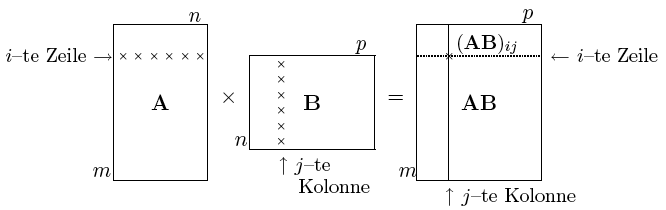
\includegraphics[width=\textwidth]{img/matrix_multiplikation.png}
        	\begin{align*}
        		c_{ij} & :\equiv \sum_{k=1}^{n} a_{ik} b_{kj} \\
        		& = a_{i1} b_{1j} + a_{i2} b_{2j} + \cdots + a_{in} b_{nj} \\
        		&\mathrel{\phantom{=}} \qquad (i = 1, \dots ,m; j = 1, \dots ,p) 
        	\end{align*}
        \end{falg}
    
    	
    	\textbf{Alternative Rechenart}
    	
    	\dots von links $\Rightarrow$ Zeile um Zeile:
    	
    	\[
    		\mathbf{EA} =
    		\begin{pmatrix}
				1 & 4 & 0\\
				0 & 1 & 0\\
				0 & 0 & 1
 			\end{pmatrix}
 			\begin{pmatrix}
				3 & 7 & 5 \\
				4 & 5 & 1 \\
				2 & 0 & 3
			\end{pmatrix}
    	\]
    	
    	Die erste Zeile von $\mathbf{EA}$ setzt sich nach der ersten Zeile von 
    	$\mathbf{E}$ zusammen: 
    	\[
    		(\mathbf{E})_{1i} = (1 \quad 4 \quad 0) 
    			\quad (\text{mit } i = 1,\dots ,3)
    	\]
    	1 mal aus der ersten Zeile von $\mA$ und 4 mal aus der zweiten
    	Zeile von $\mA$ (und 0 mal der dritten Zeile).
		
		\begin{align*}
			(\mathbf{EA})_{1j} & = e_{11} \mathbf{a}_{1j} + e_{12} \mathbf{a}_{2j}
				+ e_{13} \mathbf{a}_{3j} \\
			& = 1 \ (3 \quad 7 \quad 5) + 4 \ (4 \quad 5 \quad 1) 
				+ 0 \ (2 \quad 0 \quad 3) \\
			& = (3 \quad 7 \quad 5) + (16 \quad 20 \quad 4) \\
			& = (19 \quad 27 \quad 9) \\
			&\mathrel{\phantom{=}} \qquad (\text{mit } j = 1,\dots ,3)
		\end{align*}
		
		\[
			\mathbf{EA} =
			\begin{pmatrix}
				19 & 77 & 9 \\
				4 & 5 & 1 \\
				2 & 0 & 3
			\end{pmatrix}
		\]
		
		\textit{Multiplikation von rechts analog.}
		
		\subsubsection{Rechenregeln}
		
		\begin{frules}%[Rechenregeln]
			
			\[
				\mA \mB \not= \mB \mA
			\]
			
			\centering{(allgemein; sonst kommutativ \& symetrisch)}
			
			% Aus Satz 2.1
			\begin{align*}
				% (\alpha \beta)\mA &= \alpha (\beta \mA) \\
				(\alpha \mA)\mB & = \alpha (\mA \mB) = \mA(\alpha \mB) \\
				(\alpha + \beta)\mA & = (\alpha \mA) + (\beta \mA) \\
				\alpha(\mA + \mB) & = (\alpha \mA) + (\alpha \mB) \\
				\mA + \mB &= \mB + \mA &&\text{(Add.kommutativ)}\\
				(\mA + \mB) + \mC & = \mA + (\mB + \mC) &&\text{(Add. assoziativ)}\\
				(\mA \mB)\mC & = \mA (\mB \mC) &&\text{(Mult. assoziativ)}\\
				(\mA + \mB)\mC & = (\mA \mC) + (\mB \mC) \\
				\mA(\mB + \mC) & = (\mA \mB) + (\mA \mC) \\
				\\
				\mathbf{x} \alpha & :\equiv \mathbf{x}(\alpha) = \alpha \mathbf{x} \\
				\\
				(\mA \mB)^T = \mB^T \mA^T \ &; \ (\mA \mB)^H = \mB^H \mA^H
			\end{align*}
	
		\end{frules}
	
	
	\subsection{Transponierte einer Matrix}
	
		\begin{fdef}[Normalfall $\mA^T$]
		
			Zeilen und Spalten vertauschen:
			\[
				\begin{pmatrix}
				        1 & 2 & 3\\
				        4 & 5 & 6
				\end{pmatrix}^T
				= 
				\begin{pmatrix}
					1 & 4\\
					2 & 5\\
					3 & 6
				\end{pmatrix}
			\]
			
		\end{fdef}
		
		\begin{fdef}[$\mA$ besitzt komplexe Einträge]
		
			Hat $\mA$ komplexe Einträge so definiert man $\mB=\mA^H$ als die $n\times m$
			Matrix $\mB$ mit $b_{ij} = \overline{a_{ji}} \quad$  
			($\overline{\alpha + i \beta} = \alpha - i \beta$)
			\[
				\mA^H = 
				\begin{pmatrix}
					2+i & 3-i \\
					1+i & 1-i
				\end{pmatrix}^H
				=
				\begin{pmatrix}
					2-i & 1-i \\
					3+i & 1+i
				\end{pmatrix}
			\]
		\end{fdef}
			
		\begin{fsubdef}[symetrisch]
			\[
				\mA^T = \mA
			\]
			
			\textbf{schiefsymetrisch}
			\[
				\mA^T = -\mA
			\]
			$\Rightarrow$ Diagonale lauter Nullen \\
			
			\textbf{Hermitesch}
			\[
				\mA^H = \mA
			\]
			$\Rightarrow$ Diagonalelemente sind reell \\
			
			immer symetrisch:
			\[
				\mA^T \mA \text{ und } \mA \mA^T
			\]
			
		\end{fsubdef}

	\subsection{Skalarprodukt (SP)}
	
		\begin{fdef}[Skalarprodukt, inneres Produkt]
			$\langle x,y \rangle = x^H y$
		\end{fdef}
		
		\begin{fcharac}[Eigenschaften SP]
			\begin{align*}
				\langle x,y \rangle &= \overline{\langle y,x \rangle} \\
				\langle x,x \rangle &\ge 0 \\
				\langle x,ay+z \rangle &= a\langle x,y \rangle+ \langle x,z \rangle \\
				&\rightarrow \langle ax+z,y \rangle = \overline{a} \langle x,y 
					\rangle +\langle z,y \rangle
			\end{align*}
		\end{fcharac}
		
	\subsection{2-Norm (auch Länge oder Euklidsche Norm)}
	
		\begin{fdef}[2-Norm (auch Länge oder Euklidsche Norm)]
			\[
				||\mathbf{x}|| :\equiv \sqrt{\langle \mathbf{x},\mathbf{x} \rangle} 
					= \sqrt{\mathbf{x}^H \mathbf{x}}
			\]
		\end{fdef}
		
		\begin{ftheo}[Schwarsche Ungleichung]
			\[
				|\langle \mathbf{x},\mathbf{y} \rangle| \ \leq \ ||\mathbf{x}|| \ ||\mathbf{y}||
			\]
		\end{ftheo}


	
	
	
